% Useful packages
\documentclass[12pt]{article}
\usepackage[a4paper, left=0.75in, right=0.75in, top=0.75in, bottom=0.75in]{geometry}
\usepackage{amsmath}
\usepackage{amssymb}
\usepackage{float}
\usepackage{tabularx}
\usepackage{array}
\usepackage{multirow}
\usepackage{booktabs}
\usepackage{minted}
\usepackage{xcolor}
\usepackage{enumitem}
\usepackage{hyperref}
\usepackage{graphicx}
\usepackage{longtable}
\usepackage{adjustbox}
\usepackage{textcomp}
\usepackage{subcaption}
\usepackage{mathtools}


% chktex-file 13
% chktex-file 24
% chktex-file 36
% chktex-file 44


% Customizations
\definecolor{inputGray}{HTML}{f8f8f8}
\definecolor{outGray}{HTML}{dfdfdf}


\title{%
    Machine Learning in Computational Biology \\
    \Large Assignment 1 \\
    Bonus Questions
    }
\author{%
    Konstantinos Konstantinidis \\
    Student number: 7115152400017
    }

\begin{document}

\maketitle

\vspace{0.5in}

\textbf{\underline{Repo:}} The repository for this assignment can be found here: \\
\url{https://github.com/KonsKons26/Assignment-1}

\vspace{0.5in}

% \clearpage
% Table of contents
\tableofcontents


\clearpage
%%%%%%%%%%%%%%%%%%%%%%%%%%%%%%%%%%%%%%%%%%%%%%%%%%%%%%%%%%%%%%%%%%%%%%%%%%%%%%%%%%%%
%%%%%%%%%%%%%%%%%%%%%%%%%%%%%%%%%%%%%%%%%%%%%%%%%%%%%%%%%%%%%%%%%%%%%%%%%%%%%%%%%%%%
\section{First bonus task: Using Optuna for hyperparameter tuning}


%%%%%%%%%%%%%%%%%%%%%%%%%%%%%%%%%%%%%%%%%%%%%%%%%%%%%%%%%%%%%%%%%%%%%%%%%%%%%%%%%%%%
\subsection{Migration to Optuna}
Since the \texttt{Regressor} object I had created to perform all regression tasks
was highly modularized, with specific methods for each task, moving from \texttt{%
sklearn}'s \texttt{GridSearchCV} to \texttt{Optuna} was quite simple. I created
a new class named \texttt{RegressorOptuna} which inherited from \texttt{Regressor},
to keep it's basic functionalities the same. Then I modified the private methods
handling each model's hyperparameter optimization to allow me to pass the appropriate
grid spaces --and in the appropriate format-- for \texttt{Optuna} to tune the models.

The objective function \textbf{minimizes} the RMSE of the test set. The sampler
I chose is the \texttt{TPESampler}, a tree-structured Parzen estimator, which fits
one Gaussian Mixture Model (GMM) ($l{x}$) to the set of parameters associated with
the best objective values and another GMM ($g(x)$) to the remaining parameter values.
It chooses the parameter that minimizes the ration $l(x)/g(x)$.

All files are in the appropriate directories, \texttt{src/} and \texttt{notebooks/}
and the models were saved in \texttt{models/bonus1\_optuna/}. Since I used the
features I selected in the previous task, to keep everything organized, the process
includes copying the features files in the \texttt{models/bonus1\_optuna}
directory.

%%%%%%%%%%%%%%%%%%%%%%%%%%%%%%%%%%%%%%%%%%%%%%%%%%%%%%%%%%%%%%%%%%%%%%%%%%%%%%%%%%%%
\subsection{Hyperparameter tuning}
I set the number of trials for each model tuning to $1000$, which seemed appropriate,
as it was not such a demanding number for my machine, and since the hyperparameter
space has so many dimension, I believe that a small number of trials might not be
enough to search the whole space. The complete hyperparameter space, along with the
values chosen by \texttt{Optuna} are shown in Table~\ref{tab:hyperparams}.

\begin{table}[H]
    \centering
    \begin{tabular}{|c|c|c|c|}
        \hline
        \textbf{Model} & \textbf{Parameter} & \textbf{Values} & \textbf{Picked value} \\
        \hline
        \multirow{3}{*}{ElasticNet} 
            & \texttt{$\alpha$} & (0.01, 1.0) & $0.9998$ \\
            & \texttt{l1 ratio} & (0.0, 1.0) & $0.00004$ \\
            & \texttt{tolerance} & [1e-3, 1e-4, 1e-5, 1e-6, 1e-7] & $0.0001$ \\
        \hline
        \multirow{7}{*}{SVR} 
            & \texttt{kernel} & [`rbf', `linear', `poly', `sigmoid'] & `rbf' \\
            & \texttt{degree} & (2, 5) & $2$ \\
            & \texttt{$\gamma$} & [`scale', `auto'] & `auto' \\
            & \texttt{coef\_0} & (0.0, 1) & $0.46631$ \\
            & \texttt{tolerance} & [1e-3, 1e-4, 1e-5, 1e-6, 1e-7] & 1e-6 \\
            & \texttt{C} & (0.1, 10) & $1.49583$ \\
            & \texttt{$\epsilon$} & (0.0, 10.0) & $0.10783$ \\
        \hline
        \multirow{6}{*}{BayesianRidge} 
            & \texttt{tolerance} & [1e-3, 1e-4, 1e-5, 1e-6, 1e-7] & 1e-3 \\
            & \texttt{$\alpha_1$} & (1e-9, 1e-3) & $0.00001$ \\
            & \texttt{$\alpha_2$} & (1e-9, 1e-3) & $0.0$ \\
            & \texttt{$\lambda_1$} & (1e-3, 1e-9) & $0.0$ \\
            & \texttt{$\lambda_2$} & (1e-3, 1e-9) & $0.001$ \\
            & \texttt{compute\_score} & [True, False] & True \\
        \hline
    \end{tabular}
    \caption{Hyperparameter spaces for each model.}
    \label{tab:hyperparams}
\end{table}

%%%%%%%%%%%%%%%%%%%%%%%%%%%%%%%%%%%%%%%%%%%%%%%%%%%%%%%%%%%%%%%%%%%%%%%%%%%%%%%%%%%%
\subsection{Results}
After tuning, the best models were saved (along with their scalers, like in the
previous task) and then the validation set was used to measure their performance.
For testing, the same approach with resampling was followed, for $1000$ repeats.
The resulting boxplots are shown in Figure~\ref{fig:optuna}.

\begin{figure}[H]
    \centering
    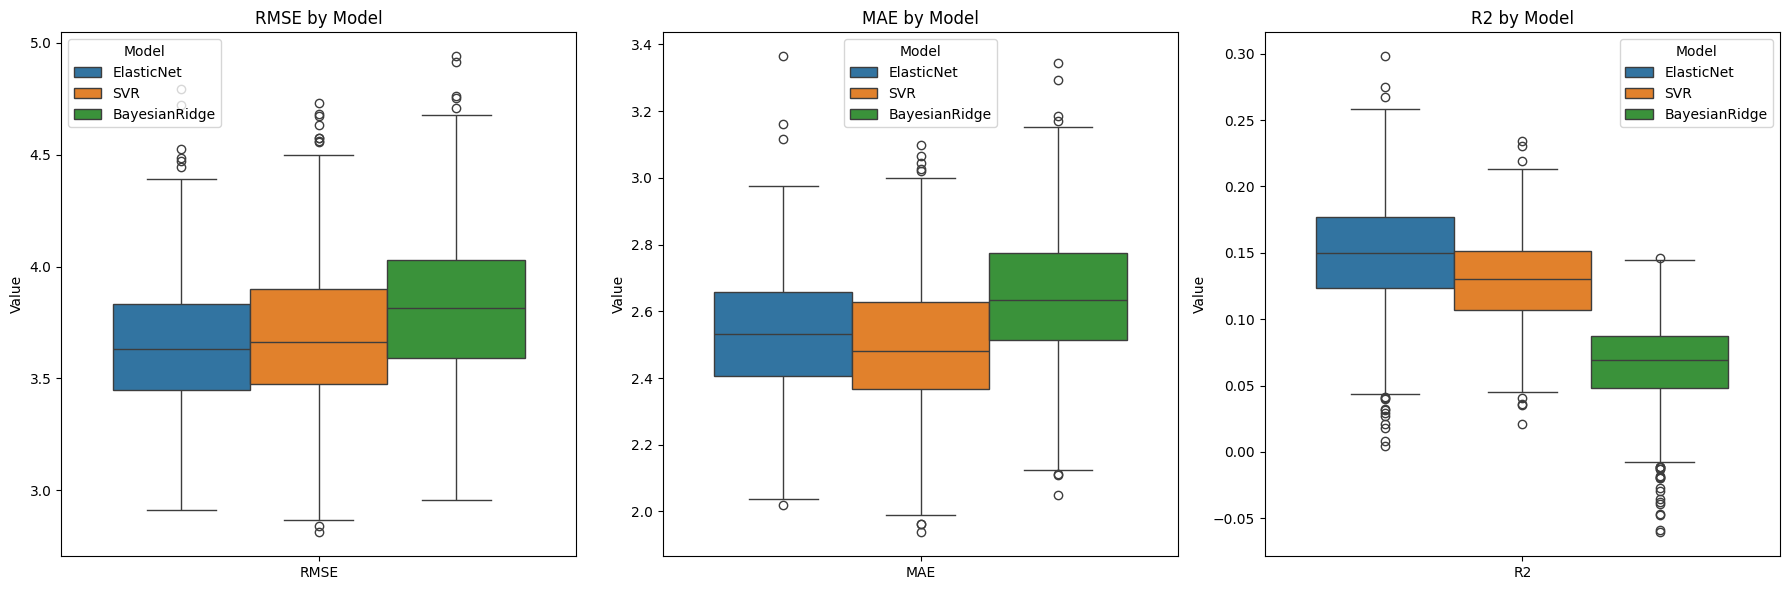
\includegraphics[width=\textwidth]{ims/optuna.png}
    \caption{Test metrics after tuning with \texttt{Optuna}. ElasticNet in blue,
    SVR in orange, and Bayesian Ridge in green.}
    \label{fig:optuna}
\end{figure}

Similar to what was shown in the previous task, Elastic Net is the best performing
model, but its RMSE and MAE still fail to drop below $3$, while $r^2$ fails to
overcome $0.2$. These findings further increase my confidence that this dataset
can not be used for regression tasks, at least no with the models that we analyzed.


\clearpage
%%%%%%%%%%%%%%%%%%%%%%%%%%%%%%%%%%%%%%%%%%%%%%%%%%%%%%%%%%%%%%%%%%%%%%%%%%%%%%%%%%%%
%%%%%%%%%%%%%%%%%%%%%%%%%%%%%%%%%%%%%%%%%%%%%%%%%%%%%%%%%%%%%%%%%%%%%%%%%%%%%%%%%%%%
\section{Second bonus task: Converting the problem to a binary classification task}




\end{document}